
% Default to the notebook output style

    


% Inherit from the specified cell style.




    
\documentclass[11pt]{article}

    
    
    \usepackage[T1]{fontenc}
    % Nicer default font (+ math font) than Computer Modern for most use cases
    \usepackage{mathpazo}

    % Basic figure setup, for now with no caption control since it's done
    % automatically by Pandoc (which extracts ![](path) syntax from Markdown).
    \usepackage{graphicx}
    % We will generate all images so they have a width \maxwidth. This means
    % that they will get their normal width if they fit onto the page, but
    % are scaled down if they would overflow the margins.
    \makeatletter
    \def\maxwidth{\ifdim\Gin@nat@width>\linewidth\linewidth
    \else\Gin@nat@width\fi}
    \makeatother
    \let\Oldincludegraphics\includegraphics
    % Set max figure width to be 80% of text width, for now hardcoded.
    \renewcommand{\includegraphics}[1]{\Oldincludegraphics[width=.8\maxwidth]{#1}}
    % Ensure that by default, figures have no caption (until we provide a
    % proper Figure object with a Caption API and a way to capture that
    % in the conversion process - todo).
    \usepackage{caption}
    \DeclareCaptionLabelFormat{nolabel}{}
    \captionsetup{labelformat=nolabel}

    \usepackage{adjustbox} % Used to constrain images to a maximum size 
    \usepackage{xcolor} % Allow colors to be defined
    \usepackage{enumerate} % Needed for markdown enumerations to work
    \usepackage{geometry} % Used to adjust the document margins
    \usepackage{amsmath} % Equations
    \usepackage{amssymb} % Equations
    \usepackage{textcomp} % defines textquotesingle
    % Hack from http://tex.stackexchange.com/a/47451/13684:
    \AtBeginDocument{%
        \def\PYZsq{\textquotesingle}% Upright quotes in Pygmentized code
    }
    \usepackage{upquote} % Upright quotes for verbatim code
    \usepackage{eurosym} % defines \euro
    \usepackage[mathletters]{ucs} % Extended unicode (utf-8) support
    \usepackage[utf8x]{inputenc} % Allow utf-8 characters in the tex document
    \usepackage{fancyvrb} % verbatim replacement that allows latex
    \usepackage{grffile} % extends the file name processing of package graphics 
                         % to support a larger range 
    % The hyperref package gives us a pdf with properly built
    % internal navigation ('pdf bookmarks' for the table of contents,
    % internal cross-reference links, web links for URLs, etc.)
    \usepackage{hyperref}
    \usepackage{longtable} % longtable support required by pandoc >1.10
    \usepackage{booktabs}  % table support for pandoc > 1.12.2
    \usepackage[inline]{enumitem} % IRkernel/repr support (it uses the enumerate* environment)
    \usepackage[normalem]{ulem} % ulem is needed to support strikethroughs (\sout)
                                % normalem makes italics be italics, not underlines
    

    
    
    % Colors for the hyperref package
    \definecolor{urlcolor}{rgb}{0,.145,.698}
    \definecolor{linkcolor}{rgb}{.71,0.21,0.01}
    \definecolor{citecolor}{rgb}{.12,.54,.11}

    % ANSI colors
    \definecolor{ansi-black}{HTML}{3E424D}
    \definecolor{ansi-black-intense}{HTML}{282C36}
    \definecolor{ansi-red}{HTML}{E75C58}
    \definecolor{ansi-red-intense}{HTML}{B22B31}
    \definecolor{ansi-green}{HTML}{00A250}
    \definecolor{ansi-green-intense}{HTML}{007427}
    \definecolor{ansi-yellow}{HTML}{DDB62B}
    \definecolor{ansi-yellow-intense}{HTML}{B27D12}
    \definecolor{ansi-blue}{HTML}{208FFB}
    \definecolor{ansi-blue-intense}{HTML}{0065CA}
    \definecolor{ansi-magenta}{HTML}{D160C4}
    \definecolor{ansi-magenta-intense}{HTML}{A03196}
    \definecolor{ansi-cyan}{HTML}{60C6C8}
    \definecolor{ansi-cyan-intense}{HTML}{258F8F}
    \definecolor{ansi-white}{HTML}{C5C1B4}
    \definecolor{ansi-white-intense}{HTML}{A1A6B2}

    % commands and environments needed by pandoc snippets
    % extracted from the output of `pandoc -s`
    \providecommand{\tightlist}{%
      \setlength{\itemsep}{0pt}\setlength{\parskip}{0pt}}
    \DefineVerbatimEnvironment{Highlighting}{Verbatim}{commandchars=\\\{\}}
    % Add ',fontsize=\small' for more characters per line
    \newenvironment{Shaded}{}{}
    \newcommand{\KeywordTok}[1]{\textcolor[rgb]{0.00,0.44,0.13}{\textbf{{#1}}}}
    \newcommand{\DataTypeTok}[1]{\textcolor[rgb]{0.56,0.13,0.00}{{#1}}}
    \newcommand{\DecValTok}[1]{\textcolor[rgb]{0.25,0.63,0.44}{{#1}}}
    \newcommand{\BaseNTok}[1]{\textcolor[rgb]{0.25,0.63,0.44}{{#1}}}
    \newcommand{\FloatTok}[1]{\textcolor[rgb]{0.25,0.63,0.44}{{#1}}}
    \newcommand{\CharTok}[1]{\textcolor[rgb]{0.25,0.44,0.63}{{#1}}}
    \newcommand{\StringTok}[1]{\textcolor[rgb]{0.25,0.44,0.63}{{#1}}}
    \newcommand{\CommentTok}[1]{\textcolor[rgb]{0.38,0.63,0.69}{\textit{{#1}}}}
    \newcommand{\OtherTok}[1]{\textcolor[rgb]{0.00,0.44,0.13}{{#1}}}
    \newcommand{\AlertTok}[1]{\textcolor[rgb]{1.00,0.00,0.00}{\textbf{{#1}}}}
    \newcommand{\FunctionTok}[1]{\textcolor[rgb]{0.02,0.16,0.49}{{#1}}}
    \newcommand{\RegionMarkerTok}[1]{{#1}}
    \newcommand{\ErrorTok}[1]{\textcolor[rgb]{1.00,0.00,0.00}{\textbf{{#1}}}}
    \newcommand{\NormalTok}[1]{{#1}}
    
    % Additional commands for more recent versions of Pandoc
    \newcommand{\ConstantTok}[1]{\textcolor[rgb]{0.53,0.00,0.00}{{#1}}}
    \newcommand{\SpecialCharTok}[1]{\textcolor[rgb]{0.25,0.44,0.63}{{#1}}}
    \newcommand{\VerbatimStringTok}[1]{\textcolor[rgb]{0.25,0.44,0.63}{{#1}}}
    \newcommand{\SpecialStringTok}[1]{\textcolor[rgb]{0.73,0.40,0.53}{{#1}}}
    \newcommand{\ImportTok}[1]{{#1}}
    \newcommand{\DocumentationTok}[1]{\textcolor[rgb]{0.73,0.13,0.13}{\textit{{#1}}}}
    \newcommand{\AnnotationTok}[1]{\textcolor[rgb]{0.38,0.63,0.69}{\textbf{\textit{{#1}}}}}
    \newcommand{\CommentVarTok}[1]{\textcolor[rgb]{0.38,0.63,0.69}{\textbf{\textit{{#1}}}}}
    \newcommand{\VariableTok}[1]{\textcolor[rgb]{0.10,0.09,0.49}{{#1}}}
    \newcommand{\ControlFlowTok}[1]{\textcolor[rgb]{0.00,0.44,0.13}{\textbf{{#1}}}}
    \newcommand{\OperatorTok}[1]{\textcolor[rgb]{0.40,0.40,0.40}{{#1}}}
    \newcommand{\BuiltInTok}[1]{{#1}}
    \newcommand{\ExtensionTok}[1]{{#1}}
    \newcommand{\PreprocessorTok}[1]{\textcolor[rgb]{0.74,0.48,0.00}{{#1}}}
    \newcommand{\AttributeTok}[1]{\textcolor[rgb]{0.49,0.56,0.16}{{#1}}}
    \newcommand{\InformationTok}[1]{\textcolor[rgb]{0.38,0.63,0.69}{\textbf{\textit{{#1}}}}}
    \newcommand{\WarningTok}[1]{\textcolor[rgb]{0.38,0.63,0.69}{\textbf{\textit{{#1}}}}}
    
    
    % Define a nice break command that doesn't care if a line doesn't already
    % exist.
    \def\br{\hspace*{\fill} \\* }
    % Math Jax compatability definitions
    \def\gt{>}
    \def\lt{<}
    % Document parameters
    \title{Applications of Convex.jl in Optimization Involving Complex Numbers}
    
    
    

    % Pygments definitions
    
\makeatletter
\def\PY@reset{\let\PY@it=\relax \let\PY@bf=\relax%
    \let\PY@ul=\relax \let\PY@tc=\relax%
    \let\PY@bc=\relax \let\PY@ff=\relax}
\def\PY@tok#1{\csname PY@tok@#1\endcsname}
\def\PY@toks#1+{\ifx\relax#1\empty\else%
    \PY@tok{#1}\expandafter\PY@toks\fi}
\def\PY@do#1{\PY@bc{\PY@tc{\PY@ul{%
    \PY@it{\PY@bf{\PY@ff{#1}}}}}}}
\def\PY#1#2{\PY@reset\PY@toks#1+\relax+\PY@do{#2}}

\expandafter\def\csname PY@tok@gd\endcsname{\def\PY@tc##1{\textcolor[rgb]{0.63,0.00,0.00}{##1}}}
\expandafter\def\csname PY@tok@gu\endcsname{\let\PY@bf=\textbf\def\PY@tc##1{\textcolor[rgb]{0.50,0.00,0.50}{##1}}}
\expandafter\def\csname PY@tok@gt\endcsname{\def\PY@tc##1{\textcolor[rgb]{0.00,0.27,0.87}{##1}}}
\expandafter\def\csname PY@tok@gs\endcsname{\let\PY@bf=\textbf}
\expandafter\def\csname PY@tok@gr\endcsname{\def\PY@tc##1{\textcolor[rgb]{1.00,0.00,0.00}{##1}}}
\expandafter\def\csname PY@tok@cm\endcsname{\let\PY@it=\textit\def\PY@tc##1{\textcolor[rgb]{0.25,0.50,0.50}{##1}}}
\expandafter\def\csname PY@tok@vg\endcsname{\def\PY@tc##1{\textcolor[rgb]{0.10,0.09,0.49}{##1}}}
\expandafter\def\csname PY@tok@vi\endcsname{\def\PY@tc##1{\textcolor[rgb]{0.10,0.09,0.49}{##1}}}
\expandafter\def\csname PY@tok@vm\endcsname{\def\PY@tc##1{\textcolor[rgb]{0.10,0.09,0.49}{##1}}}
\expandafter\def\csname PY@tok@mh\endcsname{\def\PY@tc##1{\textcolor[rgb]{0.40,0.40,0.40}{##1}}}
\expandafter\def\csname PY@tok@cs\endcsname{\let\PY@it=\textit\def\PY@tc##1{\textcolor[rgb]{0.25,0.50,0.50}{##1}}}
\expandafter\def\csname PY@tok@ge\endcsname{\let\PY@it=\textit}
\expandafter\def\csname PY@tok@vc\endcsname{\def\PY@tc##1{\textcolor[rgb]{0.10,0.09,0.49}{##1}}}
\expandafter\def\csname PY@tok@il\endcsname{\def\PY@tc##1{\textcolor[rgb]{0.40,0.40,0.40}{##1}}}
\expandafter\def\csname PY@tok@go\endcsname{\def\PY@tc##1{\textcolor[rgb]{0.53,0.53,0.53}{##1}}}
\expandafter\def\csname PY@tok@cp\endcsname{\def\PY@tc##1{\textcolor[rgb]{0.74,0.48,0.00}{##1}}}
\expandafter\def\csname PY@tok@gi\endcsname{\def\PY@tc##1{\textcolor[rgb]{0.00,0.63,0.00}{##1}}}
\expandafter\def\csname PY@tok@gh\endcsname{\let\PY@bf=\textbf\def\PY@tc##1{\textcolor[rgb]{0.00,0.00,0.50}{##1}}}
\expandafter\def\csname PY@tok@ni\endcsname{\let\PY@bf=\textbf\def\PY@tc##1{\textcolor[rgb]{0.60,0.60,0.60}{##1}}}
\expandafter\def\csname PY@tok@nl\endcsname{\def\PY@tc##1{\textcolor[rgb]{0.63,0.63,0.00}{##1}}}
\expandafter\def\csname PY@tok@nn\endcsname{\let\PY@bf=\textbf\def\PY@tc##1{\textcolor[rgb]{0.00,0.00,1.00}{##1}}}
\expandafter\def\csname PY@tok@no\endcsname{\def\PY@tc##1{\textcolor[rgb]{0.53,0.00,0.00}{##1}}}
\expandafter\def\csname PY@tok@na\endcsname{\def\PY@tc##1{\textcolor[rgb]{0.49,0.56,0.16}{##1}}}
\expandafter\def\csname PY@tok@nb\endcsname{\def\PY@tc##1{\textcolor[rgb]{0.00,0.50,0.00}{##1}}}
\expandafter\def\csname PY@tok@nc\endcsname{\let\PY@bf=\textbf\def\PY@tc##1{\textcolor[rgb]{0.00,0.00,1.00}{##1}}}
\expandafter\def\csname PY@tok@nd\endcsname{\def\PY@tc##1{\textcolor[rgb]{0.67,0.13,1.00}{##1}}}
\expandafter\def\csname PY@tok@ne\endcsname{\let\PY@bf=\textbf\def\PY@tc##1{\textcolor[rgb]{0.82,0.25,0.23}{##1}}}
\expandafter\def\csname PY@tok@nf\endcsname{\def\PY@tc##1{\textcolor[rgb]{0.00,0.00,1.00}{##1}}}
\expandafter\def\csname PY@tok@si\endcsname{\let\PY@bf=\textbf\def\PY@tc##1{\textcolor[rgb]{0.73,0.40,0.53}{##1}}}
\expandafter\def\csname PY@tok@s2\endcsname{\def\PY@tc##1{\textcolor[rgb]{0.73,0.13,0.13}{##1}}}
\expandafter\def\csname PY@tok@nt\endcsname{\let\PY@bf=\textbf\def\PY@tc##1{\textcolor[rgb]{0.00,0.50,0.00}{##1}}}
\expandafter\def\csname PY@tok@nv\endcsname{\def\PY@tc##1{\textcolor[rgb]{0.10,0.09,0.49}{##1}}}
\expandafter\def\csname PY@tok@s1\endcsname{\def\PY@tc##1{\textcolor[rgb]{0.73,0.13,0.13}{##1}}}
\expandafter\def\csname PY@tok@dl\endcsname{\def\PY@tc##1{\textcolor[rgb]{0.73,0.13,0.13}{##1}}}
\expandafter\def\csname PY@tok@ch\endcsname{\let\PY@it=\textit\def\PY@tc##1{\textcolor[rgb]{0.25,0.50,0.50}{##1}}}
\expandafter\def\csname PY@tok@m\endcsname{\def\PY@tc##1{\textcolor[rgb]{0.40,0.40,0.40}{##1}}}
\expandafter\def\csname PY@tok@gp\endcsname{\let\PY@bf=\textbf\def\PY@tc##1{\textcolor[rgb]{0.00,0.00,0.50}{##1}}}
\expandafter\def\csname PY@tok@sh\endcsname{\def\PY@tc##1{\textcolor[rgb]{0.73,0.13,0.13}{##1}}}
\expandafter\def\csname PY@tok@ow\endcsname{\let\PY@bf=\textbf\def\PY@tc##1{\textcolor[rgb]{0.67,0.13,1.00}{##1}}}
\expandafter\def\csname PY@tok@sx\endcsname{\def\PY@tc##1{\textcolor[rgb]{0.00,0.50,0.00}{##1}}}
\expandafter\def\csname PY@tok@bp\endcsname{\def\PY@tc##1{\textcolor[rgb]{0.00,0.50,0.00}{##1}}}
\expandafter\def\csname PY@tok@c1\endcsname{\let\PY@it=\textit\def\PY@tc##1{\textcolor[rgb]{0.25,0.50,0.50}{##1}}}
\expandafter\def\csname PY@tok@fm\endcsname{\def\PY@tc##1{\textcolor[rgb]{0.00,0.00,1.00}{##1}}}
\expandafter\def\csname PY@tok@o\endcsname{\def\PY@tc##1{\textcolor[rgb]{0.40,0.40,0.40}{##1}}}
\expandafter\def\csname PY@tok@kc\endcsname{\let\PY@bf=\textbf\def\PY@tc##1{\textcolor[rgb]{0.00,0.50,0.00}{##1}}}
\expandafter\def\csname PY@tok@c\endcsname{\let\PY@it=\textit\def\PY@tc##1{\textcolor[rgb]{0.25,0.50,0.50}{##1}}}
\expandafter\def\csname PY@tok@mf\endcsname{\def\PY@tc##1{\textcolor[rgb]{0.40,0.40,0.40}{##1}}}
\expandafter\def\csname PY@tok@err\endcsname{\def\PY@bc##1{\setlength{\fboxsep}{0pt}\fcolorbox[rgb]{1.00,0.00,0.00}{1,1,1}{\strut ##1}}}
\expandafter\def\csname PY@tok@mb\endcsname{\def\PY@tc##1{\textcolor[rgb]{0.40,0.40,0.40}{##1}}}
\expandafter\def\csname PY@tok@ss\endcsname{\def\PY@tc##1{\textcolor[rgb]{0.10,0.09,0.49}{##1}}}
\expandafter\def\csname PY@tok@sr\endcsname{\def\PY@tc##1{\textcolor[rgb]{0.73,0.40,0.53}{##1}}}
\expandafter\def\csname PY@tok@mo\endcsname{\def\PY@tc##1{\textcolor[rgb]{0.40,0.40,0.40}{##1}}}
\expandafter\def\csname PY@tok@kd\endcsname{\let\PY@bf=\textbf\def\PY@tc##1{\textcolor[rgb]{0.00,0.50,0.00}{##1}}}
\expandafter\def\csname PY@tok@mi\endcsname{\def\PY@tc##1{\textcolor[rgb]{0.40,0.40,0.40}{##1}}}
\expandafter\def\csname PY@tok@kn\endcsname{\let\PY@bf=\textbf\def\PY@tc##1{\textcolor[rgb]{0.00,0.50,0.00}{##1}}}
\expandafter\def\csname PY@tok@cpf\endcsname{\let\PY@it=\textit\def\PY@tc##1{\textcolor[rgb]{0.25,0.50,0.50}{##1}}}
\expandafter\def\csname PY@tok@kr\endcsname{\let\PY@bf=\textbf\def\PY@tc##1{\textcolor[rgb]{0.00,0.50,0.00}{##1}}}
\expandafter\def\csname PY@tok@s\endcsname{\def\PY@tc##1{\textcolor[rgb]{0.73,0.13,0.13}{##1}}}
\expandafter\def\csname PY@tok@kp\endcsname{\def\PY@tc##1{\textcolor[rgb]{0.00,0.50,0.00}{##1}}}
\expandafter\def\csname PY@tok@w\endcsname{\def\PY@tc##1{\textcolor[rgb]{0.73,0.73,0.73}{##1}}}
\expandafter\def\csname PY@tok@kt\endcsname{\def\PY@tc##1{\textcolor[rgb]{0.69,0.00,0.25}{##1}}}
\expandafter\def\csname PY@tok@sc\endcsname{\def\PY@tc##1{\textcolor[rgb]{0.73,0.13,0.13}{##1}}}
\expandafter\def\csname PY@tok@sb\endcsname{\def\PY@tc##1{\textcolor[rgb]{0.73,0.13,0.13}{##1}}}
\expandafter\def\csname PY@tok@sa\endcsname{\def\PY@tc##1{\textcolor[rgb]{0.73,0.13,0.13}{##1}}}
\expandafter\def\csname PY@tok@k\endcsname{\let\PY@bf=\textbf\def\PY@tc##1{\textcolor[rgb]{0.00,0.50,0.00}{##1}}}
\expandafter\def\csname PY@tok@se\endcsname{\let\PY@bf=\textbf\def\PY@tc##1{\textcolor[rgb]{0.73,0.40,0.13}{##1}}}
\expandafter\def\csname PY@tok@sd\endcsname{\let\PY@it=\textit\def\PY@tc##1{\textcolor[rgb]{0.73,0.13,0.13}{##1}}}

\def\PYZbs{\char`\\}
\def\PYZus{\char`\_}
\def\PYZob{\char`\{}
\def\PYZcb{\char`\}}
\def\PYZca{\char`\^}
\def\PYZam{\char`\&}
\def\PYZlt{\char`\<}
\def\PYZgt{\char`\>}
\def\PYZsh{\char`\#}
\def\PYZpc{\char`\%}
\def\PYZdl{\char`\$}
\def\PYZhy{\char`\-}
\def\PYZsq{\char`\'}
\def\PYZdq{\char`\"}
\def\PYZti{\char`\~}
% for compatibility with earlier versions
\def\PYZat{@}
\def\PYZlb{[}
\def\PYZrb{]}
\makeatother


    % Exact colors from NB
    \definecolor{incolor}{rgb}{0.0, 0.0, 0.5}
    \definecolor{outcolor}{rgb}{0.545, 0.0, 0.0}



    
    % Prevent overflowing lines due to hard-to-break entities
    \sloppy 
    % Setup hyperref package
    \hypersetup{
      breaklinks=true,  % so long urls are correctly broken across lines
      colorlinks=true,
      urlcolor=urlcolor,
      linkcolor=linkcolor,
      citecolor=citecolor,
      }
    % Slightly bigger margins than the latex defaults
    
    \geometry{verbose,tmargin=1in,bmargin=1in,lmargin=1in,rmargin=1in}
    
    

    \begin{document}
    
    
    \maketitle
    
    

    
    \section{Applications of Convex.jl in Optimization Involving Complex
Numbers}\label{applications-of-convex.jl-in-optimization-involving-complex-numbers}

\subsection{Ayush Pandey \textbar{} JuliaCon
2017}\label{ayush-pandey-juliacon-2017}

\url{https://github.com/Ayush-iitkgp/JuliaCon2017Presentation}

    \section{About Me}\label{about-me}

\begin{itemize}
\item
  \textbf{BS and MS in Mathematics and Computing Sciences
  (July'12-June'17) at Indian Institute of Technology Kharagpur }
\item
  \textbf{Google Summer of Code 2016 and 2017 student under the Julia
  Language}
\item
  \textbf{GitHub:} \href{https://github.com/ayush-iitkgp}{Ayush-iitkgp}
\item
  \textbf{Website:}
  \href{https://ayush-iitkgp.github.io/}{https://ayush-iitkgp.github.io}
\end{itemize}

    \section{Outline}\label{outline}

\begin{itemize}
\tightlist
\item
  Power Flow Optimization
\item
  Fidelity in Quantum Information 
\end{itemize}

    \subsubsection{Optimal Power Flow -
Introduction}\label{optimal-power-flow---introduction}

\begin{itemize}
\tightlist
\item
  Power flow study is an analysis of a connected electrical power
  system's capability to adequately supply the connected load.
\end{itemize}

\begin{figure}
\centering
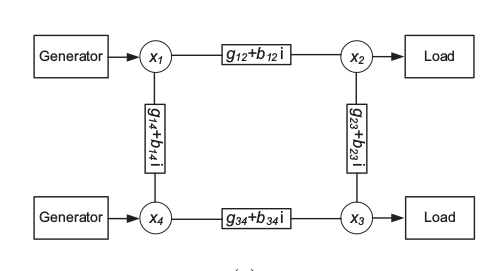
\includegraphics{Power_Network.png}
\caption{An example of a power network}
\end{figure}

\begin{itemize}
\tightlist
\item
  \textbf{Unknowns: } - Voltages angle and magnitude information for
  each bus
\item
  \textbf{Knowns: } - Load( such as appliances and lights.) and
  generator real power and voltage condition. 
\end{itemize}

    \subsubsection{Optimal Power Flow - Mathematical
Formulation}\label{optimal-power-flow---mathematical-formulation}

    \paragraph{Constraints}\label{constraints}

\begin{figure}
\centering
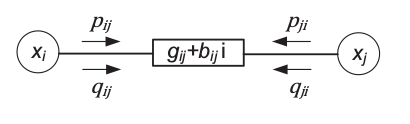
\includegraphics{Power_Network_2.png}
\caption{Each transmission line has four flows}
\end{figure}

\begin{itemize}
\tightlist
\item
  \(p_{ij}\): Active power entering the line from node i
\item
  \(q_{ij}\): Reactive power entering the line from node i
\item
  Let \(x_{i}\) denote the complex voltage for node i of the network.
\end{itemize}

We have the following power balance equations which are
\textbf{non-linear} in unknown \(x_{i}\) and \(x_{j}\).

\begin{figure}
\centering
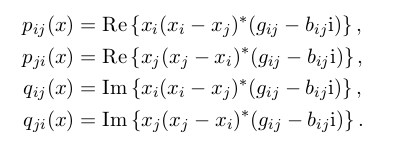
\includegraphics{Power_Network_3.png}
\caption{Power balance equations}
\end{figure}

    \paragraph{Objective}\label{objective}

Depends upon the business needs such as:

\begin{itemize}
\tightlist
\item
  Minimize power losses in an electrical network
\item
  Minimize cost of generation
\end{itemize}

    \subsubsection{Optimal Power Flow - SDP
Relaxation}\label{optimal-power-flow---sdp-relaxation}

\begin{itemize}
\tightlist
\item
  The original optimal power flow problem is non-convex in nature.
\item
  Thanks to the
  \href{https://www.informs.org/content/download/320453/3031884/version/2/file/OStoday2016.pdf}{\textbf{lifting
  technique}} which converts the above optimization problem to a
  SemiDefinite Programming Problem.
\item
  The relaxed SDP problem finds the \textbf{near global solution} of the
  original non-convex problem.
\end{itemize}

    \subsubsection{Example}\label{example}

\begin{itemize}
\tightlist
\item
  The data is taken from the IEEE 14 Bus test case which represents a
  portion of the American Electric Power System (in the Midwestern US)
  as of February, 1962.
\end{itemize}

    \begin{Verbatim}[commandchars=\\\{\}]
{\color{incolor}In [{\color{incolor}37}]:} \PY{k}{using} \PY{n}{Convex}  \PY{c}{\PYZsh{} Read the input data}
         \PY{k}{using} \PY{n}{FactCheck}
         \PY{k}{using} \PY{n}{MAT}   \PY{c}{\PYZsh{}Pkg.add(\PYZdq{}MAT\PYZdq{})}
         \PY{n}{TOL} \PY{o}{=} \PY{l+m+mf}{1e\PYZhy{}2}\PY{p}{;}
         \PY{n}{input} \PY{o}{=} \PY{n}{matopen}\PY{p}{(}\PY{l+s}{\PYZdq{}}\PY{l+s}{D}\PY{l+s}{a}\PY{l+s}{t}\PY{l+s}{a}\PY{l+s}{.}\PY{l+s}{m}\PY{l+s}{a}\PY{l+s}{t}\PY{l+s}{\PYZdq{}}\PY{p}{)}
         \PY{n}{varnames} \PY{o}{=} \PY{n}{names}\PY{p}{(}\PY{n}{input}\PY{p}{)}
         \PY{n}{Data} \PY{o}{=} \PY{n}{read}\PY{p}{(}\PY{n}{input}\PY{p}{,} \PY{l+s}{\PYZdq{}}\PY{l+s}{i}\PY{l+s}{n}\PY{l+s}{j}\PY{l+s}{\PYZdq{}}\PY{p}{,}\PY{l+s}{\PYZdq{}}\PY{l+s}{Y}\PY{l+s}{\PYZdq{}}\PY{p}{)}\PY{p}{;}
         \PY{n}{n}\PY{o}{=}\PY{n}{size}\PY{p}{(}\PY{n}{Data}\PY{p}{[}\PY{l+m+mi}{2}\PY{p}{]}\PY{p}{,}\PY{l+m+mi}{1}\PY{p}{)}\PY{p}{;} \PY{c}{\PYZsh{} Create some intermediate variables}
         \PY{n}{Y}\PY{o}{=}\PY{n}{Data}\PY{p}{[}\PY{l+m+mi}{2}\PY{p}{]}\PY{p}{;}
         \PY{n}{inj}\PY{o}{=}\PY{n}{Data}\PY{p}{[}\PY{l+m+mi}{1}\PY{p}{]}\PY{p}{;}
\end{Verbatim}


    \begin{Verbatim}[commandchars=\\\{\}]
{\color{incolor}In [{\color{incolor}38}]:} \PY{n}{W} \PY{o}{=} \PY{n}{ComplexVariable}\PY{p}{(}\PY{n}{n}\PY{p}{,}\PY{n}{n}\PY{p}{)}\PY{p}{;} \PY{c}{\PYZsh{} W is the matrix of pairwise products of the voltages}
         
         \PY{n}{objective} \PY{o}{=} \PY{n}{real}\PY{p}{(}\PY{n}{sum}\PY{p}{(}\PY{n}{diag}\PY{p}{(}\PY{n}{W}\PY{p}{)}\PY{p}{)}\PY{p}{)}\PY{p}{;} \PY{c}{\PYZsh{} The objective is to minimize cost of generation}
         
         \PY{n}{c1} \PY{o}{=} \PY{n}{Constraint}\PY{p}{[}\PY{p}{]}\PY{p}{;} \PY{c}{\PYZsh{} The constraints are power balance equations}
         \PY{k}{for} \PY{n}{i}\PY{o}{=}\PY{l+m+mi}{2}\PY{o}{:}\PY{n}{n}
             \PY{n}{push!}\PY{p}{(}\PY{n}{c1}\PY{p}{,}\PY{n}{sum}\PY{p}{(}\PY{n}{W}\PY{p}{[}\PY{n}{i}\PY{p}{,}\PY{o}{:}\PY{p}{]}\PY{o}{.*}\PY{p}{(}\PY{n}{Y}\PY{p}{[}\PY{n}{i}\PY{p}{,}\PY{o}{:}\PY{p}{]}\PY{o}{\PYZsq{}}\PY{p}{)}\PY{p}{)}\PY{o}{==}\PY{n}{inj}\PY{p}{[}\PY{n}{i}\PY{p}{]}\PY{p}{)}\PY{p}{;}
         \PY{k}{end}
         \PY{n}{c2} \PY{o}{=} \PY{n}{W} \PY{k+kp}{in} \PY{o}{:}\PY{n}{SDP}\PY{p}{;}
         \PY{n}{c3} \PY{o}{=} \PY{n}{real}\PY{p}{(}\PY{n}{W}\PY{p}{[}\PY{l+m+mi}{1}\PY{p}{,}\PY{l+m+mi}{1}\PY{p}{]}\PY{p}{)}\PY{o}{==}\PY{l+m+mf}{1.06}\PY{o}{\PYZca{}}\PY{l+m+mi}{2}\PY{p}{;}
         \PY{n}{push!}\PY{p}{(}\PY{n}{c1}\PY{p}{,} \PY{n}{c2}\PY{p}{)}\PY{p}{;}
         \PY{n}{push!}\PY{p}{(}\PY{n}{c1}\PY{p}{,} \PY{n}{c3}\PY{p}{)}\PY{p}{;}
\end{Verbatim}


    \begin{Verbatim}[commandchars=\\\{\}]
{\color{incolor}In [{\color{incolor}39}]:} \PY{n}{p} \PY{o}{=} \PY{n}{maximize}\PY{p}{(}\PY{n}{objective}\PY{p}{,}\PY{n}{c1}\PY{p}{)}\PY{p}{;} \PY{c}{\PYZsh{} Create the problem}
         \PY{n}{solve!}\PY{p}{(}\PY{n}{p}\PY{p}{)}\PY{p}{;} \PY{c}{\PYZsh{} Solve the problem}
         \PY{n}{p}\PY{o}{.}\PY{n}{optval} \PY{c}{\PYZsh{}15.125857662600703}
         \PY{n}{evaluate}\PY{p}{(}\PY{n}{objective}\PY{p}{)} \PY{c}{\PYZsh{}15.1258578588357}
\end{Verbatim}


    \begin{Verbatim}[commandchars=\\\{\}]
----------------------------------------------------------------------------
	SCS v1.2.6 - Splitting Conic Solver
	(c) Brendan O'Donoghue, Stanford University, 2012-2016
----------------------------------------------------------------------------
Lin-sys: sparse-direct, nnz in A = 1344
eps = 1.00e-04, alpha = 1.80, max\_iters = 20000, normalize = 1, scale = 5.00
Variables n = 393, constraints m = 812
Cones:	primal zero / dual free vars: 406
	sd vars: 406, sd blks: 1
Setup time: 6.53e-04s
----------------------------------------------------------------------------
 Iter | pri res | dua res | rel gap | pri obj | dua obj | kap/tau | time (s)
----------------------------------------------------------------------------
     0|      inf       inf      -nan      -inf       inf       inf  3.16e-04 
   100| 3.92e-02  8.28e-02  6.88e-05 -1.43e+01 -1.43e+01  1.23e-16  1.01e-01 
   200| 7.31e-03  1.97e-02  1.66e-05 -1.48e+01 -1.48e+01  0.00e+00  1.61e-01 
   300| 2.71e-03  5.88e-03  5.13e-06 -1.50e+01 -1.50e+01  1.27e-16  2.24e-01 
   400| 8.98e-04  1.92e-03  1.68e-06 -1.51e+01 -1.51e+01  1.27e-16  2.73e-01 
   500| 2.88e-04  6.27e-04  5.46e-07 -1.51e+01 -1.51e+01  1.27e-16  3.30e-01 
   600| 9.25e-05  2.02e-04  1.75e-07 -1.51e+01 -1.51e+01  1.27e-16  3.98e-01 
   680| 3.73e-05  8.15e-05  7.03e-08 -1.51e+01 -1.51e+01  1.27e-16  4.39e-01 
----------------------------------------------------------------------------
Status: Solved
Timing: Solve time: 4.39e-01s
	Lin-sys: nnz in L factor: 2906, avg solve time: 1.97e-05s
	Cones: avg projection time: 6.13e-04s
----------------------------------------------------------------------------
Error metrics:
dist(s, K) = 2.1500e-09, dist(y, K*) = 2.0328e-09, s'y/|s||y| = 3.5844e-13
|Ax + s - b|\_2 / (1 + |b|\_2) = 3.7310e-05
|A'y + c|\_2 / (1 + |c|\_2) = 8.1457e-05
|c'x + b'y| / (1 + |c'x| + |b'y|) = 7.0266e-08
----------------------------------------------------------------------------
c'x = -15.1259, -b'y = -15.1259
============================================================================

    \end{Verbatim}

    \begin{Verbatim}[commandchars=\\\{\}]
{\color{incolor}In [{\color{incolor}40}]:} \PY{n}{output} \PY{o}{=} \PY{n}{matopen}\PY{p}{(}\PY{l+s}{\PYZdq{}}\PY{l+s}{R}\PY{l+s}{e}\PY{l+s}{s}\PY{l+s}{.}\PY{l+s}{m}\PY{l+s}{a}\PY{l+s}{t}\PY{l+s}{\PYZdq{}}\PY{p}{)}\PY{p}{;} \PY{c}{\PYZsh{} Verify the results}
         \PY{n}{names}\PY{p}{(}\PY{n}{output}\PY{p}{)}\PY{p}{;}
         \PY{n}{outputData} \PY{o}{=} \PY{n}{read}\PY{p}{(}\PY{n}{output}\PY{p}{,} \PY{l+s}{\PYZdq{}}\PY{l+s}{W}\PY{l+s}{r}\PY{l+s}{e}\PY{l+s}{s}\PY{l+s}{\PYZdq{}}\PY{p}{)}\PY{p}{;}
         \PY{n}{Wres} \PY{o}{=} \PY{n}{outputData}\PY{p}{;}
         \PY{n}{real\PYZus{}diff} \PY{o}{=} \PY{n}{real}\PY{p}{(}\PY{n}{W}\PY{o}{.}\PY{n}{value}\PY{p}{)} \PY{o}{\PYZhy{}} \PY{n}{real}\PY{p}{(}\PY{n}{Wres}\PY{p}{)}\PY{p}{;}
         \PY{n}{imag\PYZus{}diff} \PY{o}{=} \PY{n}{imag}\PY{p}{(}\PY{n}{W}\PY{o}{.}\PY{n}{value}\PY{p}{)} \PY{o}{\PYZhy{}} \PY{n}{imag}\PY{p}{(}\PY{n}{Wres}\PY{p}{)}\PY{p}{;}
         \PY{n+nd}{@fact} \PY{n}{real\PYZus{}diff} \PY{o}{=\PYZgt{}} \PY{n}{roughly}\PY{p}{(}\PY{n}{zeros}\PY{p}{(}\PY{n}{n}\PY{p}{,}\PY{n}{n}\PY{p}{)}\PY{p}{,} \PY{n}{TOL}\PY{p}{)}\PY{p}{;}
         \PY{n+nd}{@fact} \PY{n}{imag\PYZus{}diff} \PY{o}{=\PYZgt{}} \PY{n}{roughly}\PY{p}{(}\PY{n}{zeros}\PY{p}{(}\PY{n}{n}\PY{p}{,}\PY{n}{n}\PY{p}{)}\PY{p}{,} \PY{n}{TOL}\PY{p}{)}
\end{Verbatim}


\begin{Verbatim}[commandchars=\\\{\}]
{\color{outcolor}Out[{\color{outcolor}40}]:} Success :: (line:441) :: fact was true
           Expression: imag\_diff --> roughly(zeros(n,n),TOL)
             Expected: [0.0 0.0 0.0 0.0 0.0 0.0 0.0 0.0 0.0 0.0 0.0 0.0 0.0 0.0; 0.0 0.0 0.0 0.0 0.0 0.0 0.0 0.0 0.0 0.0 0.0 0.0 0.0 0.0; 0.0 0.0 0.0 0.0 0.0 0.0 0.0 0.0 0.0 0.0 0.0 0.0 0.0 0.0; 0.0 0.0 0.0 0.0 0.0 0.0 0.0 0.0 0.0 0.0 0.0 0.0 0.0 0.0; 0.0 0.0 0.0 0.0 0.0 0.0 0.0 0.0 0.0 0.0 0.0 0.0 0.0 0.0; 0.0 0.0 0.0 0.0 0.0 0.0 0.0 0.0 0.0 0.0 0.0 0.0 0.0 0.0; 0.0 0.0 0.0 0.0 0.0 0.0 0.0 0.0 0.0 0.0 0.0 0.0 0.0 0.0; 0.0 0.0 0.0 0.0 0.0 0.0 0.0 0.0 0.0 0.0 0.0 0.0 0.0 0.0; 0.0 0.0 0.0 0.0 0.0 0.0 0.0 0.0 0.0 0.0 0.0 0.0 0.0 0.0; 0.0 0.0 0.0 0.0 0.0 0.0 0.0 0.0 0.0 0.0 0.0 0.0 0.0 0.0; 0.0 0.0 0.0 0.0 0.0 0.0 0.0 0.0 0.0 0.0 0.0 0.0 0.0 0.0; 0.0 0.0 0.0 0.0 0.0 0.0 0.0 0.0 0.0 0.0 0.0 0.0 0.0 0.0; 0.0 0.0 0.0 0.0 0.0 0.0 0.0 0.0 0.0 0.0 0.0 0.0 0.0 0.0; 0.0 0.0 0.0 0.0 0.0 0.0 0.0 0.0 0.0 0.0 0.0 0.0 0.0 0.0]
             Occurred: [7.21891e-9 1.09908e-5 2.03142e-5 2.4322e-5 2.20655e-5 4.88765e-5 4.56099e-5 4.65576e-5 5.22527e-5 5.33708e-5 5.16477e-5 5.00836e-5 5.00343e-5 5.11381e-5; -1.09704e-5 -2.9351e-8 8.63911e-6 1.36025e-5 1.14299e-5 3.7428e-5 3.48544e-5 3.57447e-5 4.15345e-5 4.28357e-5 4.07829e-5 3.88891e-5 3.89983e-5 4.04856e-5; -2.03103e-5 -8.60839e-6 -7.09979e-8 6.05066e-6 3.72136e-6 2.97453e-5 2.77659e-5 2.8529e-5 3.47725e-5 3.63289e-5 3.3859e-5 3.15844e-5 3.18855e-5 3.38928e-5; -2.43209e-5 -1.35708e-5 -6.00392e-6 -3.13606e-7 -1.88926e-6 2.24612e-5 2.07537e-5 2.16031e-5 2.73258e-5 2.88318e-5 2.64326e-5 2.41747e-5 2.44664e-5 2.63617e-5; -2.20443e-5 -1.14021e-5 -3.72034e-6 2.07534e-6 -1.84344e-7 2.45569e-5 2.2733e-5 2.35753e-5 2.92654e-5 3.07001e-5 2.83942e-5 2.62314e-5 2.64812e-5 2.82721e-5; -4.88785e-5 -3.74309e-5 -2.97522e-5 -2.24708e-5 -2.44784e-5 -3.87313e-7 -9.82969e-7 -3.40895e-7 6.05173e-6 7.85915e-6 4.97049e-6 2.29021e-6 2.84209e-6 5.35518e-6; -4.56128e-5 -3.48578e-5 -2.77738e-5 -2.0657e-5 -2.2739e-5 9.68386e-7 -4.80534e-7 8.06184e-7 6.77224e-6 8.3796e-6 5.60517e-6 3.03697e-6 3.50253e-6 5.87174e-6; -4.65526e-5 -3.57413e-5 -2.85295e-5 -2.16068e-5 -2.35738e-5 3.33978e-7 -6.39029e-7 -1.27845e-7 6.01353e-6 7.704e-6 4.94367e-6 2.40328e-6 2.85565e-6 5.2099e-6; -5.22657e-5 -4.1548e-5 -3.47903e-5 -2.72942e-5 -2.92814e-5 -6.07701e-6 -6.44929e-6 -6.03233e-6 -7.73445e-7 1.95546e-6 -1.16352e-6 -3.87795e-6 -3.33431e-6 -7.19737e-7; -5.33756e-5 -4.28413e-5 -3.63384e-5 -2.88447e-5 -3.07081e-5 -7.87585e-6 -8.39717e-6 -7.71444e-6 -1.56187e-6 -4.75029e-7 -2.84532e-6 -5.68387e-6 -5.12984e-6 -2.56324e-6; -5.16454e-5 -4.07821e-5 -3.38616e-5 -2.64385e-5 -2.83949e-5 -4.84957e-6 -5.61542e-6 -4.94684e-6 1.14314e-6 3.00238e-6 -2.2845e-7 -2.71874e-6 -2.17579e-6 3.97771e-7; -5.00789e-5 -3.88847e-5 -3.15841e-5 -2.41781e-5 -2.62298e-5 -2.20113e-6 -3.04454e-6 -2.40263e-6 3.86015e-6 5.6745e-6 2.71626e-6 -1.22655e-7 5.7586e-7 3.1552e-6; -5.00336e-5 -3.89984e-5 -3.18895e-5 -2.44736e-5 -2.64833e-5 -2.66205e-6 -3.51414e-6 -2.85949e-6 3.31239e-6 5.11613e-6 2.16904e-6 -5.15582e-7 -2.69548e-7 2.61995e-6; -5.11346e-5 -4.04833e-5 -3.38943e-5 -2.6366e-5 -2.82716e-5 -5.36328e-6 -5.88052e-6 -5.21155e-6 8.19018e-7 2.5525e-6 -4.01939e-7 -3.15624e-6 -2.53924e-6 -1.62076e-7]
\end{Verbatim}
            
    \subsubsection{Fidelity in Quantum Information Theory -
Introduction}\label{fidelity-in-quantum-information-theory---introduction}

\begin{itemize}
\item
  This example is inspired from a lecture of John Watrous in the
  \href{https://cs.uwaterloo.ca/~watrous/CS766/LectureNotes/08.pdf}{course
  on Theory of Quantum Information}.
\item
  Fidelity is a measure of the \textbf{closeness} of two quantum states.
\item
  The ability to distinguish between the quantum states is equivalent to
  the ability to distinguish between the classical probability
  distributions.
\item
  If fidelity between two states is 1, they are the same quantum state.
\end{itemize}

    \begin{itemize}
\tightlist
\item
  \textbf{Application}
\end{itemize}

\begin{figure}
\centering
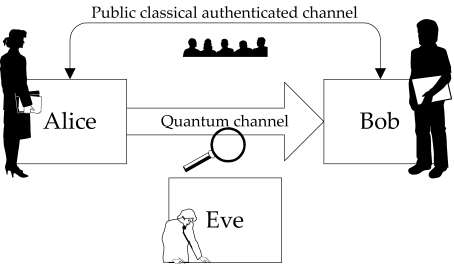
\includegraphics{Fidelity.png}
\caption{Quantum Cryptography}
\end{figure}

\begin{itemize}
\tightlist
\item
  The Fidelity between two Hermitian semidefinite matrices P and Q is
  defined as:
\end{itemize}

\[F(P,Q) = {||{P}^{1/2}{Q}^{1/2} ||}_{tr} =  \max\; |trace({P}^{1/2}U{Q}^{1/2})|\]

where the trace norm \(||.||_{tr}\) is the sum of the singular values,
and the maximization goes over the set of all unitary matrices U.

    \subsubsection{Fidelity in Quantum Information Theory - Mathematical
Formulation}\label{fidelity-in-quantum-information-theory---mathematical-formulation}

Fidelity can be expressed as the optimal value of the following
complex-valued SDP:

\[ \textbf{maximize} \frac{1}{2} trace(Z+Z^*)\]

\[\text{subject to } \left[\begin{array}{cc}P&Z\\{Z}^{*}&Q\end{array}\right] \succeq 0\]

\[\text{where } Z \in \mathbf {C}^{n \times n}\]

    \subsubsection{Example}\label{example}

    \begin{Verbatim}[commandchars=\\\{\}]
{\color{incolor}In [{\color{incolor}46}]:} \PY{n}{n} \PY{o}{=} \PY{l+m+mi}{20} \PY{c}{\PYZsh{} Create the data}
         \PY{n}{P} \PY{o}{=} \PY{n}{randn}\PY{p}{(}\PY{n}{n}\PY{p}{,}\PY{n}{n}\PY{p}{)} \PY{o}{+} \PY{n+nb}{im}\PY{o}{*}\PY{n}{randn}\PY{p}{(}\PY{n}{n}\PY{p}{,}\PY{n}{n}\PY{p}{)}\PY{p}{;}
         \PY{n}{P} \PY{o}{=} \PY{n}{P}\PY{o}{*}\PY{n}{P}\PY{o}{\PYZsq{}}\PY{p}{;}
         \PY{n}{Q} \PY{o}{=} \PY{n}{randn}\PY{p}{(}\PY{n}{n}\PY{p}{,}\PY{n}{n}\PY{p}{)} \PY{o}{+} \PY{n+nb}{im}\PY{o}{*}\PY{n}{randn}\PY{p}{(}\PY{n}{n}\PY{p}{,}\PY{n}{n}\PY{p}{)}\PY{p}{;}
         \PY{n}{Q} \PY{o}{=} \PY{n}{Q}\PY{o}{*}\PY{n}{Q}\PY{o}{\PYZsq{}}\PY{p}{;}
         
         \PY{n}{Z} \PY{o}{=} \PY{n}{ComplexVariable}\PY{p}{(}\PY{n}{n}\PY{p}{,}\PY{n}{n}\PY{p}{)}\PY{p}{;} \PY{c}{\PYZsh{} Declare convex variable}
         
         \PY{n}{objective} \PY{o}{=} \PY{l+m+mf}{0.5}\PY{o}{*}\PY{n}{real}\PY{p}{(}\PY{n}{trace}\PY{p}{(}\PY{n}{Z}\PY{o}{+}\PY{n}{Z}\PY{o}{\PYZsq{}}\PY{p}{)}\PY{p}{)}\PY{p}{;}  \PY{c}{\PYZsh{} Specify the problem}
         \PY{n}{constraint} \PY{o}{=} \PY{p}{[}\PY{n}{P} \PY{n}{Z}\PY{p}{;}\PY{n}{Z}\PY{o}{\PYZsq{}} \PY{n}{Q}\PY{p}{]} \PY{n}{⪰} \PY{l+m+mi}{0}\PY{p}{;}
         \PY{n}{problem} \PY{o}{=} \PY{n}{maximize}\PY{p}{(}\PY{n}{objective}\PY{p}{,}\PY{n}{constraint}\PY{p}{)}\PY{p}{;}
          
         \PY{n}{solve!}\PY{p}{(}\PY{n}{problem}\PY{p}{)} \PY{c}{\PYZsh{} Solve the problem}
\end{Verbatim}


    \begin{Verbatim}[commandchars=\\\{\}]
----------------------------------------------------------------------------
	SCS v1.2.6 - Splitting Conic Solver
	(c) Brendan O'Donoghue, Stanford University, 2012-2016
----------------------------------------------------------------------------
Lin-sys: sparse-direct, nnz in A = 1621
eps = 1.00e-04, alpha = 1.80, max\_iters = 20000, normalize = 1, scale = 5.00
Variables n = 801, constraints m = 6401
Cones:	primal zero / dual free vars: 3161
	sd vars: 3240, sd blks: 1
Setup time: 1.91e-03s
----------------------------------------------------------------------------
 Iter | pri res | dua res | rel gap | pri obj | dua obj | kap/tau | time (s)
----------------------------------------------------------------------------
     0|      inf       inf      -nan      -inf      -inf       inf  7.54e-03 
   100| 1.01e-03  2.31e-01  2.50e-02 -5.66e+02 -5.39e+02  0.00e+00  2.30e-01 
   200| 2.22e-04  5.11e-02  3.54e-03 -5.75e+02 -5.71e+02  0.00e+00  4.48e-01 
   300| 7.54e-05  1.64e-02  7.96e-04 -5.75e+02 -5.74e+02  0.00e+00  6.73e-01 
   400| 3.46e-05  6.67e-03  2.29e-04 -5.75e+02 -5.75e+02  0.00e+00  9.00e-01 
   500| 1.79e-05  2.98e-03  7.65e-05 -5.75e+02 -5.75e+02  0.00e+00  1.11e+00 
   600| 9.20e-06  1.39e-03  2.84e-05 -5.75e+02 -5.75e+02  0.00e+00  1.30e+00 
   700| 4.56e-06  6.63e-04  1.16e-05 -5.75e+02 -5.75e+02  0.00e+00  1.51e+00 
   800| 2.18e-06  3.20e-04  5.17e-06 -5.75e+02 -5.75e+02  0.00e+00  1.73e+00 
   900| 1.03e-06  1.55e-04  2.42e-06 -5.75e+02 -5.75e+02  0.00e+00  1.93e+00 
   980| 5.63e-07  8.75e-05  1.35e-06 -5.75e+02 -5.75e+02  0.00e+00  2.14e+00 
----------------------------------------------------------------------------
Status: Solved
Timing: Solve time: 2.14e+00s
	Lin-sys: nnz in L factor: 8823, avg solve time: 6.83e-05s
	Cones: avg projection time: 2.04e-03s
----------------------------------------------------------------------------
Error metrics:
dist(s, K) = 3.1242e-09, dist(y, K*) = 1.1761e-09, s'y/|s||y| = -1.5744e-12
|Ax + s - b|\_2 / (1 + |b|\_2) = 5.6250e-07
|A'y + c|\_2 / (1 + |c|\_2) = 8.7453e-05
|c'x + b'y| / (1 + |c'x| + |b'y|) = 1.3527e-06
----------------------------------------------------------------------------
c'x = -575.3507, -b'y = -575.3492
============================================================================

    \end{Verbatim}

    \begin{Verbatim}[commandchars=\\\{\}]
{\color{incolor}In [{\color{incolor}47}]:} \PY{c}{\PYZsh{} Verify that computer fidelity is equal to actual fidelity}
         \PY{n}{computed\PYZus{}fidelity} \PY{o}{=} \PY{n}{evaluate}\PY{p}{(}\PY{n}{objective}\PY{p}{)}
         \PY{n}{P1}\PY{p}{,}\PY{n}{P2} \PY{o}{=} \PY{n}{eig}\PY{p}{(}\PY{n}{P}\PY{p}{)}\PY{p}{;}
         \PY{n}{sqP} \PY{o}{=} \PY{n}{P2} \PY{o}{*} \PY{n}{diagm}\PY{p}{(}\PY{p}{[}\PY{n}{p1}\PY{o}{\PYZca{}}\PY{l+m+mf}{0.5} \PY{k}{for} \PY{n}{p1} \PY{k+kp}{in} \PY{n}{P1}\PY{p}{]}\PY{p}{)} \PY{o}{*} \PY{n}{P2}\PY{o}{\PYZsq{}}
         \PY{n}{Q1}\PY{p}{,}\PY{n}{Q2} \PY{o}{=} \PY{n}{eig}\PY{p}{(}\PY{n}{Q}\PY{p}{)}
         \PY{n}{sqQ} \PY{o}{=} \PY{n}{Q2} \PY{o}{*} \PY{n}{diagm}\PY{p}{(}\PY{p}{[}\PY{n}{q1}\PY{o}{\PYZca{}}\PY{l+m+mf}{0.5} \PY{k}{for} \PY{n}{q1} \PY{k+kp}{in} \PY{n}{Q1}\PY{p}{]}\PY{p}{)} \PY{o}{*} \PY{n}{Q2}\PY{o}{\PYZsq{}}
         \PY{n}{actual\PYZus{}fidelity} \PY{o}{=} \PY{n}{sum}\PY{p}{(}\PY{n}{svd}\PY{p}{(}\PY{n}{sqP} \PY{o}{*} \PY{n}{sqQ}\PY{p}{)}\PY{p}{[}\PY{l+m+mi}{2}\PY{p}{]}\PY{p}{)}
         \PY{n}{diff} \PY{o}{=} \PY{n}{computed\PYZus{}fidelity} \PY{o}{\PYZhy{}} \PY{n}{actual\PYZus{}fidelity}
         \PY{n+nd}{@fact} \PY{n}{diff} \PY{o}{=\PYZgt{}} \PY{n}{roughly}\PY{p}{(}\PY{l+m+mi}{0}\PY{p}{,} \PY{n}{TOL}\PY{p}{)}
\end{Verbatim}


\begin{Verbatim}[commandchars=\\\{\}]
{\color{outcolor}Out[{\color{outcolor}47}]:} Success :: (line:441) :: fact was true
           Expression: diff --> roughly(0,TOL)
             Expected: 0
             Occurred: -0.0010774993736504257
\end{Verbatim}
            
    \section{Thank You!}\label{thank-you}


    % Add a bibliography block to the postdoc
    
    
    
    \end{document}
